%Anexo
\chapter{Códigos}

\section{Algoritmo}
El \hypertarget{laberinto}{algoritmo} usado para la resolución del laberinto se encuentra en el archivo \texttt{Robot.ino} y es el siguiente:
\lstinputlisting[language=C]{Robot.ino}

\section{Pruebas}
Los códigos usados para las pruebas fueron los siguientes:
\subsection{Primeras pruebas}
\hypertarget{primerasPruebas}{}
\subsubsection{Ultrasonidos}
\lstinputlisting[language=C]{Ultrasonidos.ino}
\subsubsection{Infrarrojos}
\lstinputlisting[language=C]{Infrarrojos.ino}
\subsubsection{CNY70}
\lstinputlisting[language=C]{CNY70.ino}
\subsubsection{Motores}
\lstinputlisting[language=C]{Motor.ino}
\subsubsection{Conexión bluetooth}
\lstinputlisting[language=C]{Bluetooth.ino}

\subsection{Pruebas finales}
\hypertarget{pruebasFinales}{}
\begin{lstlisting}[language=C]
// Testing code
/*
SENSORES

Serial1.print("\nDistancia delante: ");
Serial1.println(R.distanciaDelante());

Serial1.print("Distancia izquierda: ");
Serial1.println(R.distanciaIzq());

Serial1.print("Distancia derecha: ");
Serial1.println(R.distanciaDcha());

Serial1.print("CNY detras: ");
Serial1.print(R.numeroAtras());
if(R.negroAtras())
    Serial1.println(", negro");
else
    Serial1.println(", blanco");

Serial1.print("CNY izquierdo: ");
Serial1.print(R.numeroIzq());
if(R.negroIzq())
    Serial1.println(", negro");
else
    Serial1.println(", blanco");

Serial1.print("CNY derecho: ");
Serial1.print(R.numeroDcha());
if(R.negroDcha())
    Serial1.println(", negro");
else
    Serial1.println(", blanco");

delay(3000);


PAREDES

celda c = escanear(R,ultimoMuroDelante);

Serial1.print("\nDistancia delante: ");
Serial1.println(R.distanciaDelante());

if(c.delante)
    Serial1.println("Hay muro delante");
else
    Serial1.println("No hay muro delante");

Serial1.print("Distancia izquierda: ");
Serial1.println(R.distanciaIzq());

if(c.izquierda)
    Serial1.println("Hay muro izquierda");
else
    Serial1.println("No hay muro izquierda");

Serial1.print("Distancia derecha: ");
Serial1.println(R.distanciaDcha());

if(c.derecha)
    Serial1.println("Hay muro derecha");
else
    Serial1.println("No hay muro derecha");


Serial1.println("");
delay(2000);

BLUETOOTH

celda c = escanear(R,ultimoMuroDelante);

if(!c.delante)
    Serial1.print("O");
else
    Serial1.print("X");

if(!c.izquierda)
    Serial1.print("O");
else
    Serial1.print("X");

if(!c.derecha)
    Serial1.print("O");
else
    Serial1.print("X");

if(!c.detras)
    Serial1.print("O");
else
    Serial1.print("X");

if(!c.derecha)
    Serial1.print("2");

else if(!c.delante) 
    Serial1.print("0");

else if(!c.izquierda)
    Serial1.print("1");

else if(!c.detras)
    Serial1.print("3"); 
*/
\end{lstlisting}

\section{Monitorización}
\hypertarget{Monitorizacion}{}
El código para la monitorización mediante bluetooth es el siguiente:
\lstinputlisting[language=Python]{Interfazv0.9.py}

\newpage
La interfaz gráfica quedaría de así:
\begin{center}
	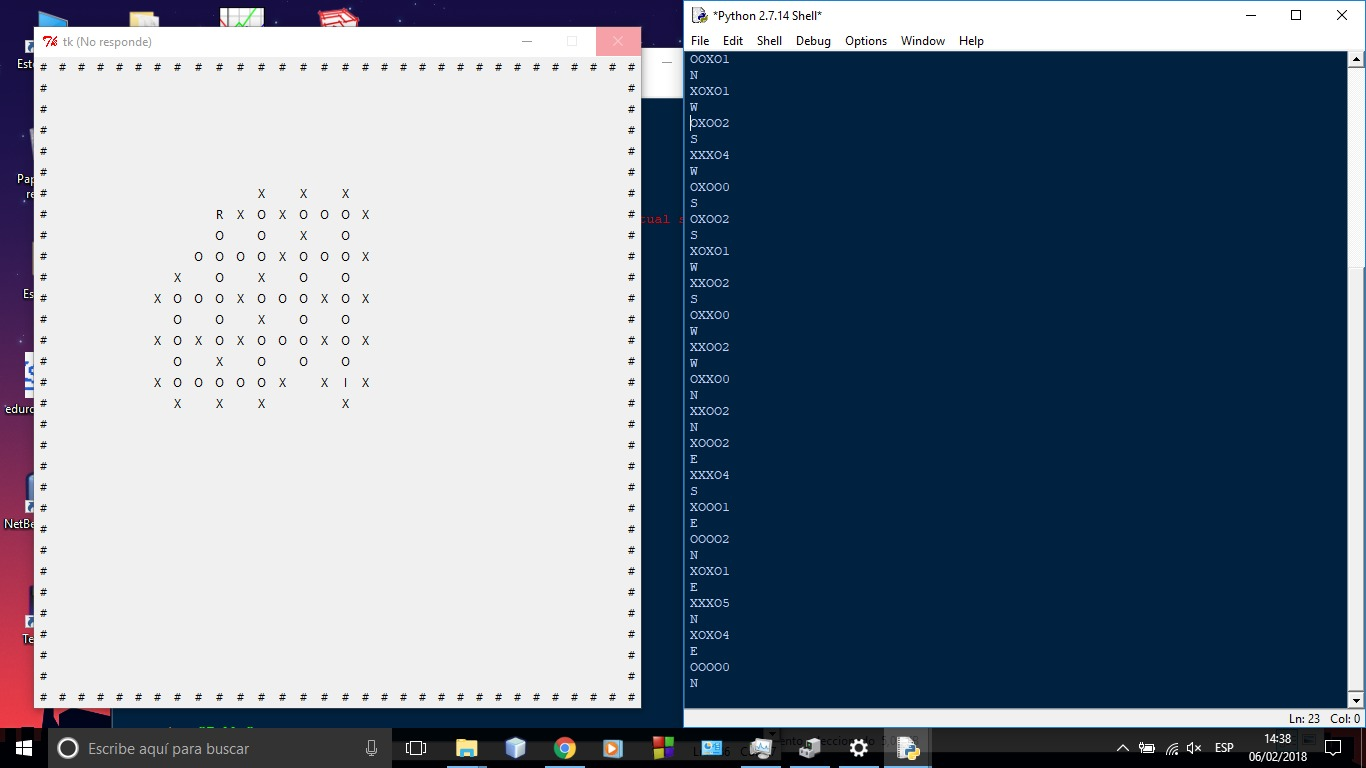
\includegraphics[scale=0.35]{Interfaz.jpeg}
\end{center}